\begin{center}
\resizebox{0.96\linewidth}{!}{%
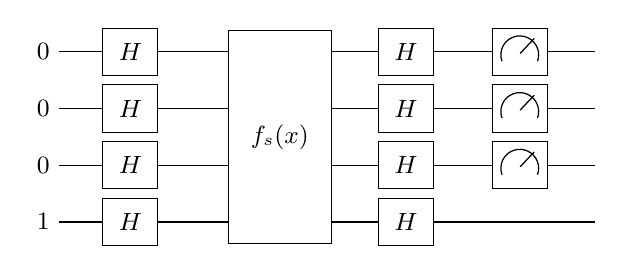
\begin{tikzpicture}[
    wire/.style={line width=0.45pt},
    gate/.style={
        draw,
        fill=white,
        minimum width=7mm,
        minimum height=6mm,
        inner sep=0pt,
        font=\small
    },
    oracle/.style={
        draw,
        fill=white,
        minimum width=13mm,
        minimum height=27mm,
        inner sep=0pt,
        font=\small,
        align=center
    },
    measure/.style={
        draw,
        fill=white,
        minimum width=7mm,
        minimum height=6mm,
        inner sep=0pt
    },
    wirelabel/.style={font=\small}
]
    \def\xstart{0}
    \def\xend{6.8}
    \foreach \y in {0,-0.72,-1.44,-2.16} {
        \draw[wire] (\xstart,\y) -- (\xend,\y);
    }

    \node[wirelabel, anchor=east] at (\xstart,0) {$\ket{0}$};
    \node[wirelabel, anchor=east] at (\xstart,-0.72) {$\ket{0}$};
    \node[wirelabel, anchor=east] at (\xstart,-1.44) {$\ket{0}$};
    \node[wirelabel, anchor=east] at (\xstart,-2.16) {$\ket{1}$};

    \node[gate] at (0.9,0) {$H$};
    \node[gate] at (0.9,-0.72) {$H$};
    \node[gate] at (0.9,-1.44) {$H$};
    \node[gate] at (0.9,-2.16) {$H$};

    \node[oracle] at (2.8,-1.08) {$f_s(\bm{x})$};

    \node[gate] at (4.4,0) {$H$};
    \node[gate] at (4.4,-0.72) {$H$};
    \node[gate] at (4.4,-1.44) {$H$};
    \node[gate] at (4.4,-2.16) {$H$};

    \foreach \y in {0,-0.72,-1.44} {
        \node[measure] at (5.85,\y) {};
        \draw[wire] (5.62,\y-0.12) arc[start angle=200, end angle=-20, radius=0.24];
        \draw[wire] (5.85,\y-0.02) -- (6.03,\y+0.17);
    }
\end{tikzpicture}%
}
\end{center}
